\documentclass{article}
\usepackage[utf8]{inputenc}
\usepackage[margin=1in]{geometry}
\usepackage{amsmath, amssymb, multicol, graphicx}
\usepackage{enumerate, enumitem, dsfont, relsize, wrapfig, bm}
\newcommand\pd{\partial}
\newcommand\bd{\mathbf}
\newcommand\curl{\nabla\times}
\usepackage{dsfont, relsize, wrapfig, bm, float, etoolbox}
\usepackage{wasysym}
\usepackage{array}
\usepackage{booktabs}
\usepackage{listings} %for formatting matlab code
\usepackage{color} %red, green, blue, yellow, cyan, magenta, black, white
\usepackage{subfigure}
\usepackage{tablefootnote}
\usepackage{multirow}
\usepackage{color} %red, green, blue, yellow, cyan, magenta, black, white
\usepackage{listings} %for formatting matlab code
\usepackage[T1]{fontenc}
\usepackage{siunitx}
\usepackage{circuitikz}
\usepackage{bigfoot} % to allow verbatim in footnote
\usepackage{pdfpages}


\usepackage{mathtools}
\DeclarePairedDelimiter\ceil{\lceil}{\rceil}
\DeclarePairedDelimiter\floor{\lfloor}{\rfloor}

\definecolor{vgreen}{RGB}{104,180,104}
\definecolor{vblue}{RGB}{49,49,255}
\definecolor{vorange}{RGB}{255,143,102}

\lstdefinestyle{verilog-style}
{
    language=Verilog,
    basicstyle=\small\ttfamily,
    keywordstyle=\color{vblue},
    identifierstyle=\color{black},
    breaklines=true,
    frame=single,
    rulecolor=\color{black},
    commentstyle=\color{vgreen},
    numbers=left,
    numberstyle=\tiny\color{black},
    numbersep=10pt,
    tabsize=4,
    moredelim=*[s][\colorIndex]{[}{]},
    literate=*{:}{:}1,
    postbreak=\mbox{\textcolor{red}{$\hookrightarrow$}\space}
}

\makeatletter
\newcommand*\@lbracket{[}
\newcommand*\@rbracket{]}
\newcommand*\@colon{:}
\newcommand*\colorIndex{%
    \edef\@temp{\the\lst@token}%
    \ifx\@temp\@lbracket \color{black}%
    \else\ifx\@temp\@rbracket \color{black}%
    \else\ifx\@temp\@colon \color{black}%
    \else \color{vorange}%
    \fi\fi\fi
}
\makeatother

\newcommand\cj{\overline}
\newcommand\xhat{\bd{\hat{x}}}
\newcommand\yhat{\bd{\hat{y}}}
\newcommand\rp{\right)}
\newcommand\lp{\left(}
\newcommand\erm{\mathrm{e}}
\newcommand\kohms{\text{ k}\Omega}
\newcommand\muA{\text{ }\mu\text{A}}

\ctikzset{bipoles/length=1cm}
\ctikzset{resistors/scale=0.7, % smaller R
 sources/scale=1,
 capacitors/scale=0.7, % even smaller C
 diodes/scale=0.6, % small diodes
 transistors/scale=1.3} % bigger BJTs

 \usepackage{fancyhdr}
 \pagestyle{fancy}
 \fancyhead[L,C]{}
 \fancyhead[L]{\textbf{\rightmark}}
 \fancyfoot[R]{ECE 111 Project --- Spring 2023}
 \fancyfoot[C]{}
 \fancyfoot[L]{Page \thepage ~of \pageref{LastPage}}
 \renewcommand{\headrulewidth}{0.4pt}
 \renewcommand{\footrulewidth}{2pt}

\begin{document}

\begin{titlepage}
   \begin{center}

       \large ECE 111: Advanced Digital Design Project \\
       Prof. Yatish Turakhia
       \vfill

       \LARGE\textbf{SHA-256 and Bitcoin Hashing Report} \\
   \vspace{0.8cm}
       \large June 10, 2023 \\

       \vfill

       Conner Hsu (A16665092) \\
       Haozhang Chu (A16484292) \\
       Kirtan Shah (A16227067)

       \date{\today}

   \end{center}
\end{titlepage}

\tableofcontents

\newpage
\section{Simplified SHA-256}

\subsection{Introduction}

% explain what SHA-256 is

Hash functions are powerful tools that play a vital role in various areas of computer science and information security. At their core, hash functions are mathematical algorithms that transform data of any size into a fixed-size string of characters, known as a hash value or hash code. This transformation is designed to have a few important properties:
\begin{itemize} %TODO some of these properties I think aren't very important for certain types of hash function use cases. I think injective, noninvertibility, and avalanche effect are only important for information security applications.
  \item compression; the output hash value is fixed in size regardless of the size of the input.
  \item avalanche effect: a small change in the input results in a huge change in the output.
  \item determinism: the same input must always generate the same output.
  \item pre-image resistant: an inverse hash function should not exist and it should be very difficult to determine the input that generated a given output.
  \item collision resistance: the hash function should be nearly completely injective and thus should almost never have two inputs map to the same output.
\end{itemize}
For cryptographic applications, avalanche effect, noninvertibility and injectiveness are very important properties. These properties all together make hash functions invaluable for tasks such as data retrieval, data integrity verification, password storage, and digital signatures. By producing unique and irreversible hash values, hash functions enable efficient data indexing, quick data comparison, and secure authentication. Whether it's ensuring data integrity, enhancing search performance, or providing robust security measures, hash functions are essential components in modern computing systems.

In this report, we explore the implementation of a particular hash function called Secure Hashing Algorithm - 256 or SHA-256 for short. This hash function takes in any length input and outputs a 256-bit digest/hash value. We will build this using System Verilog and use the Arria-II FPGA to realize the implementation on hardware.
% TODO:

\subsection{Algorithm}

% explain what SHA-256 algorithm that was implemented.

Before running the SHA-256 algorithm, the input message must be broken up into blocks of 512 bits. The final block must contain at least 66 extra bits; a 1 followed by at least one 0, and 64 bits equal to the size of the original input message. The number of zeros padding between the first 1 and the message size bits depends on how many bits are needed to make the last block 512 bits long.

For example, suppose the message is 640 bits long. This means that the first block will contain the first 512 bits of the message, and the second block will contain the last 128 bits of the message. Next, a 1 will be appended to the last block making it 129 bits long. Then, 319 zeros will be appended to make the last block now 448 bits long. Last, 64 bits will be appended to store the message size and the last block will not be 512 bits long.

As another example, suppose that the input message divides evenly into 512-bit blocks meaning that the message size is some multiple of 512. In this case, the final block will have a 1 in the beginning, then 448 zeros, then end off 64 bits for the message size. The number of zeros is increased to 448 to ensure that this final block is 512 bits long.

Throughout the SHA-256 algorithm, a set of hash values $H_0, H_1, H_2, H_3, H_4, H_5, H_6, H_7$ are updated after each block in the input message is processed. These variables are each 32 bits long and thus when put together form the 256-bit output digest.

From here, the states of the SHA-256 are described as follows. The algorithm begins in the \verb|IDLE| state. In this state, the algorithm waits for a start signal to begin computation. Once a start signal is received, it initializes iterative variables, the address to read in the input message, and the hash values, $H_i$ for $0 \leq i \leq 7$. Once this is done, the algorithm will move into the \verb|READ| state in the next clock cycle.

In the \verb|READ| state, the SHA-256 algorithm will read data from the memory read in input of the module. Since the memory module being used can only read out 32 bits (or one word) at a time, it takes multiple clock cycles before the entire input message will be read in. In our implementation, we designed the SHA-256 to take a fixed input message length of 640 bits. This means that the \verb|READ| state will use at least 20 clock cycles to read in $20\cdot 32$ bits. Once the entire input message is read in, the algorithm moves to the \verb|BLOCK| state in the next clock cycle.

In the \verb|BLOCK| state, the algorithm will separate the input message into 512-bit blocks in the same process as described earlier. For the 640-bit input message, 512 of the bits will be placed in the first block, and the last 128 bits will be placed in the second block. Some logic is needed to fill the remaining 384 bits of the second block with the zeros padding and input message size. A for-loop is used to initialize the first 10 words with $100\dots00$ and then the last two words are set to the input message size. Additionally, before moving into the next state, another set of variables, $a,b,c,d,e,f,g,h$ are initialized to the hash values from earlier. Once this is completed, the algorithm moves to the \verb|COMPUTE| state in the next clock cycle. When the algorithm is in the \verb|BLOCK| state for the first time, it will send the first 512 bits of the input message to the \verb|COMPUTE| state. When the algorithm is in the \verb|BLOCK| state of the second time, it will send the last 128 bits of the input message plus the padding and message size to the \verb|COMPUTE| state.

In the \verb|COMPUTE| state, the algorithm processes the 512-bit block. The algorithm will break these 512 bits into 16 words and then use a process called word expansion to expand this into 64 words. Each of these blocks of 32 bits are processed sequentially over 64 clock cycles. A 32-bit block along with the $a,b,c,d,e,f,g,h$ values are passed to a SHA-256 hash round function each clock cycle.

\begin{lstlisting}[style=verilog-style]
// SHA256 hash round
function logic [255:0] sha256_op(input logic [31:0] a, b, c, d, e, f, g, h, w,
    input logic [7:0] t);
  logic [31:0] S1, S0, ch, maj, t1, t2; // internal signals
  begin
    S1 = rightrotate(e, 6) ^ rightrotate(e, 11) ^ rightrotate(e, 25);
    ch = (e & f) ^ ((~e) & g);
    t1 = h + S1 + ch + k[t] + w;
    S0 = rightrotate(a, 2) ^ rightrotate(a, 13) ^ rightrotate(a, 22);
    maj = (a & b) ^ (a & c) ^ (b & c);
    t2 = S0+maj;
    sha256_op = {t1 + t2, a, b, c, d + t1, e, f, g};
  end
endfunction
\end{lstlisting}

While it is difficult to explain everything that is going on in the function, some important properties should be noted.
\begin{itemize}
  \item The AND operation is a noninvertible function if the function is not outputting 1. It is not possible to determine the inputs if the output of an AND operation is 0.
  \item The XOR operation is always noninvertible.
  \item While the function is complicated it can be realized that there is no nondeterministic processes in this function.
\end{itemize}
These properties help SHA-256 to realize properties such as determinism and pre-image resistance. After the SHA-256 hash round is complete, the output of the function will be assigned to $a,b,c,d,e,f,g,h$ and will be used in the next clock cycle. The process of updating the $a,b,c,d,e,f,g,h$ values for each word and then using the same values for the next 32-bit block helps to realize the avalanche effect. A small change in the input message will affect the output of one word, which then affects the input/output of the next 32-bit block, and will then change the inputs/outputs for all of the 32-bit blocks down the line.

Once all 64 words blocks are processed in the \verb|COMPUTE| state, the algorithm will move back to the \verb|BLOCK| state. If there are more blocks of 512 bits to be processed, then it will take the next block and move back to the \verb|COMPUTE| state. However, if there are no more blocks to be processed, then the algorithm will move to the \verb|WRITE| state.

In the \verb|WRITE| state, the algorithm will write the hash values, $H_0, H_1, H_2, H_3, H_4, H_5, H_6, H_7$ to memory. Since the memory module being used can only write 32 bits to memory per clock cycle, it will take at least 8 clock cycles to write the hash values to memory.

\iffalse
\subsection{Finer details of reading/writing from memory}

The SHA-256 uses an external memory module to read in the input message and write out the output hash. At every positive edge of clock, this memory module reads out the

%TODO: do we want to do write this section?
\fi

\subsection{Optimization}

As we will see in the next section, optimizing the SHA-256 algorithm for speed is very important. In this section, we will briefly discuss some of the changes that helped improve the maximum speed we can clock the algorithm at.

We optimized the \verb|simplified_sha256| by changing the way we assign message words and perform word expansion. First, instead of using an if statement and assigning one word per cycle to \verb|w|, we used a for-loop because it can be done in parallel. This saved about 15 cycles.
\lstinputlisting[linerange={171-184}, style=verilog-style]{simplified_sha256.sv}

We also computed the word expansion in parallel with the \verb|COMPUTE| state, which allowed us to reduce the \verb|w| register from length 64 to length 16. This saved thousands of ALUTS.
\lstinputlisting[linerange={201-212}, style=verilog-style]{simplified_sha256.sv}





\newpage
\section{Bitcoin Hashing}

\subsection{Introduction}

% explain what bitcoin hashing is

Bitcoin hashing is a critical aspect of the cryptocurrency's underlying technology, blockchain. In the context of Bitcoin, hashing refers to the process of converting transaction data into a fixed-length alphanumeric string, i.e. a hash value. In order for a block to be accepted as part of the block chain, its hash must be meet a specific criteria. Bitcoin miners must repeatedly hash different combinations of the original transaction data plus a random string of numbers called the "nonce". By changing the nonce, different hash values can be generated and Bitcoin miners will keep trying different nonces until the hash meets the specific criteria. The process of finding the nonce that meets the criteria requires a lot of computational power and since miners compete with each other to see who meets the criteria, speed is also very essential.

In this part of the report, we will investigate the implementation of a Bitcoin hashing algorithm that will attempt to generate multiple hash values at a time for different nonce values. We are not trying to meet any specific criteria for the final hash value, but instead are trying to design a module that will compute many hash values with different nonces very quickly.

\subsection{Algorithm}

% explain what bitcoin hashing algorithm that was implemented.
The goal of this algorithm is to compute 16 hash values for 16 different nonce values. Since speed is highly important in the context of Bitcoin mining, we have designed our implementation to computes these hashes as fast as possible.

This algorithm is designed to take in a 640-bit input message (read in from an external memory module similar to the SHA-256. The first 608 bits are reserved for the transaction data and the last 32 bits of the input message are reserved for the nonce. The hash function for the Bitcoin hashing is realized with the SHA-256 function from earlier. The first block of 512 bits contains the first 16 words of the transaction data. The second block contains the last 3 words of the transaction data, the word containing the nonce, and then padding and input message size. These two blocks are then processed by the SHA-256 algorithm again.

We have designed one module to process the first 512-bit block that only contains transaction data. The output hash of this module then helps to initialize the initial hash values of the SHA-256 module that processes the second block. Since we want to compute the hash values for inputs with 16 different nonce values, we ended up using 16 SHA-256 instances running in parallel to compute all 16 nonce values at once.

After output hashes are computed for both blocks of all 16 nonce values, these output hashes are then used to form a third 512-bit block for each nonce value. The first 256 bits of this block contains the hash value of the respective hash output from the first and second blocks. The last 256 bits contain padding and input message size (256). This third block is then fed into one last SHA-256 \verb|COMPUTE| state and uses the same initial hash as the one used to process the first 512-bit block.

To implement this algorithm we used multiple modules. We created a module called \verb|onephase_sha256.sv| that implements a SHA-256 algorithm that only goes through one \verb|COMPUTE| state, and another module called \verb|twophase_sha256.sv| that implements a SHA-256 algorithm that goes through the \verb|COMPUTE| state twice. Finally, a higher level module called \verb|bitcoin_hash.sv| is created to instantiate 1 one phase SHA-256 and 16 two phase SHA-256. Wires are used to connect the output hash of the one phase SHA-256 instance to the 16 instances of the two phase SHA-256.

The top-level module, \verb|bitcoin_hash.sv| handles the reading in and writing out data. This makes it so the read and write states of the one and two phase SHA-256 modules aren't necessarily required.

\subsection{Optimization}

As seen in the previous section, our proposed algorithm for Bitcoin hashing is fast since it computes all 16 hash value in parallel. Theoretically speaking, this requires the roughly the same computation time as a SHA-256 module that goes through 3 \verb|COMPUTE| states, i.e. processes 3 blocks. However, our algorithm requires implementing 17 SHA-256 instances onto the FPGA, 1 for processing the first 512-bit block and 16 for processing the second and third blocks for each nonce value. Practically speaking, the Arria-II FPGA has a difficult time fitting all 17 SHA-256 instances, so we optimized the ALUT usage.

Since we need to feed the values for \verb|h0|-\verb|h7| from phase 1, we added a parameter \verb|inh|. The input message and outputs were passed as registers as well.

\lstinputlisting[linerange={1-7}, style=verilog-style]{twophase_sha256.sv}

We were able to remove the \verb|h0|-\verb|h7| registers since \verb|a|-\verb|h| and \verb|inh| hold the final values of phase 2. This saved several thousand ALUTs.
\lstinputlisting[linerange={116-124}, style=verilog-style]{twophase_sha256.sv}

We also removed the \verb|BLOCK1| state and moved it to the \verb|IDLE| state because we can hard code the initial behavior. This eliminates the need for an if statement to decide which data to populate depending on which block we are in. This saves several thousand ALUTs. This also had the added benefit of saving a cycle.
\lstinputlisting[linerange={92-114}, style=verilog-style]{twophase_sha256.sv}

Since we are dealing with registers only, we can go directly from \verb|COMPUTE| to \verb|DONE| and output the final hash values. This saved a cycle.
\lstinputlisting[linerange={159-163}, style=verilog-style]{twophase_sha256.sv}



\subsection{Resource Usage}

% resource usage, fitter report snapshot, fmax, timing
\begin{figure}[H]
  \centering
  \begin{subfigure}
    \centering
    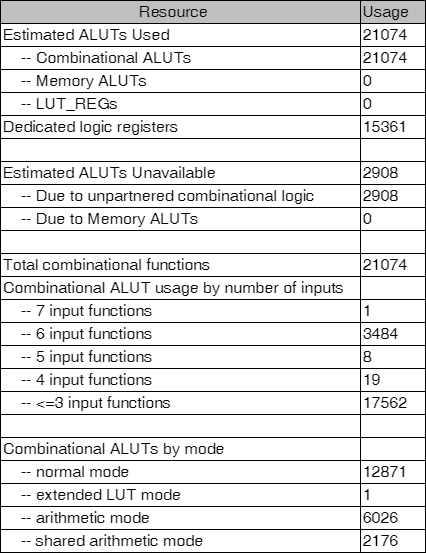
\includegraphics[width=0.45\linewidth]{r1.png}
  \end{subfigure}
  \begin{subfigure}
    \centering
    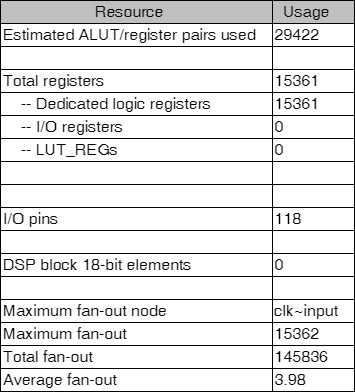
\includegraphics[width=0.45\linewidth]{r2.png}
  \end{subfigure}
  \caption{Resource usage summary for Bitcoin Hashing Module}
\end{figure}

\begin{figure}[H]
  \centering
    \centering
    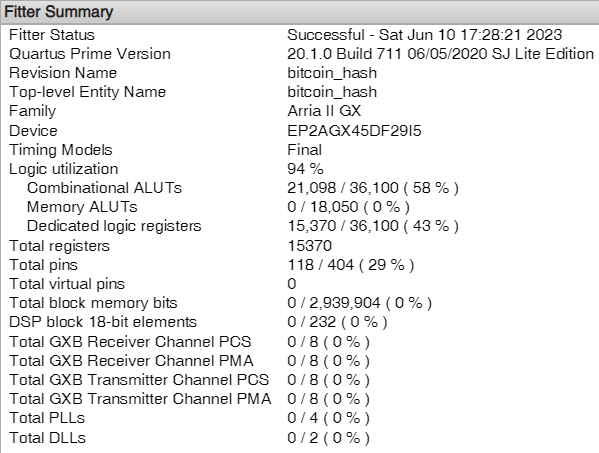
\includegraphics[width=0.7\linewidth]{fitter.png}
  \caption{Fitter report snapshot.}
\end{figure}

\begin{figure}[H]
  \centering
    \centering
    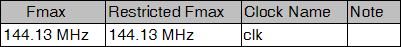
\includegraphics[width=0.6\linewidth]{fmax.png}
  \caption{$f_\text{max}$ report snapshot.}
\end{figure}

\newgeometry{
    margin=1in
}
\fancyfootoffset{0pt}
\newpage
\section{Simulation Transcripts}

\subsection{SHA-256}

\lstinputlisting[frame=single, basicstyle=\small\ttfamily,tabsize=4]{sha256.txt}

\newpage
\subsection{Bitcoin Hashing}
\lstinputlisting[frame=single, basicstyle=\small\ttfamily,tabsize=4]{bitcoin_hash.txt}

\newpage
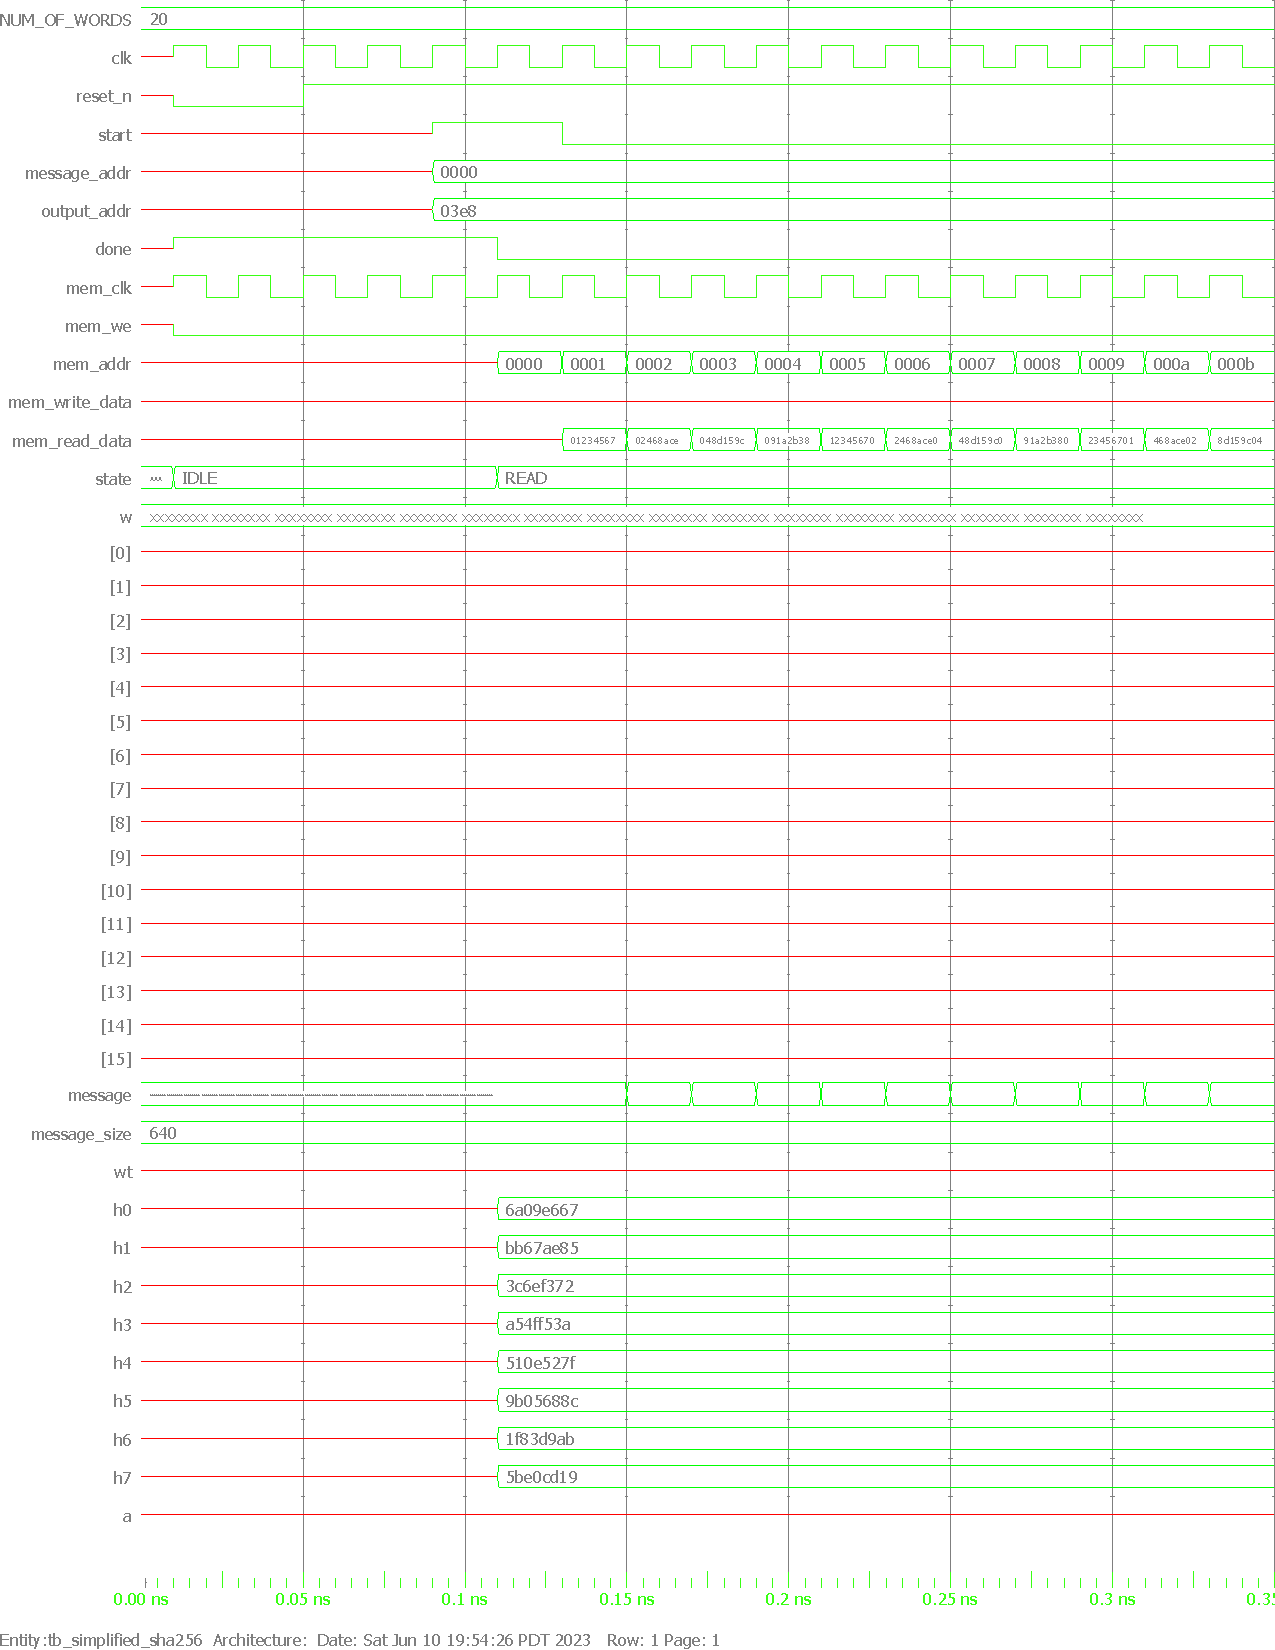
\includepdf[pages=1, pagecommand={\section{Simulation Waveforms} \subsection{SHA-256} \pagestyle{fancy}}, noautoscale = true,scale=.7]{1wave.pdf}
\includepdf[pages=2-, pagecommand={\pagestyle{fancy}}, noautoscale = true,scale=.8]{1wave.pdf}

\newpage



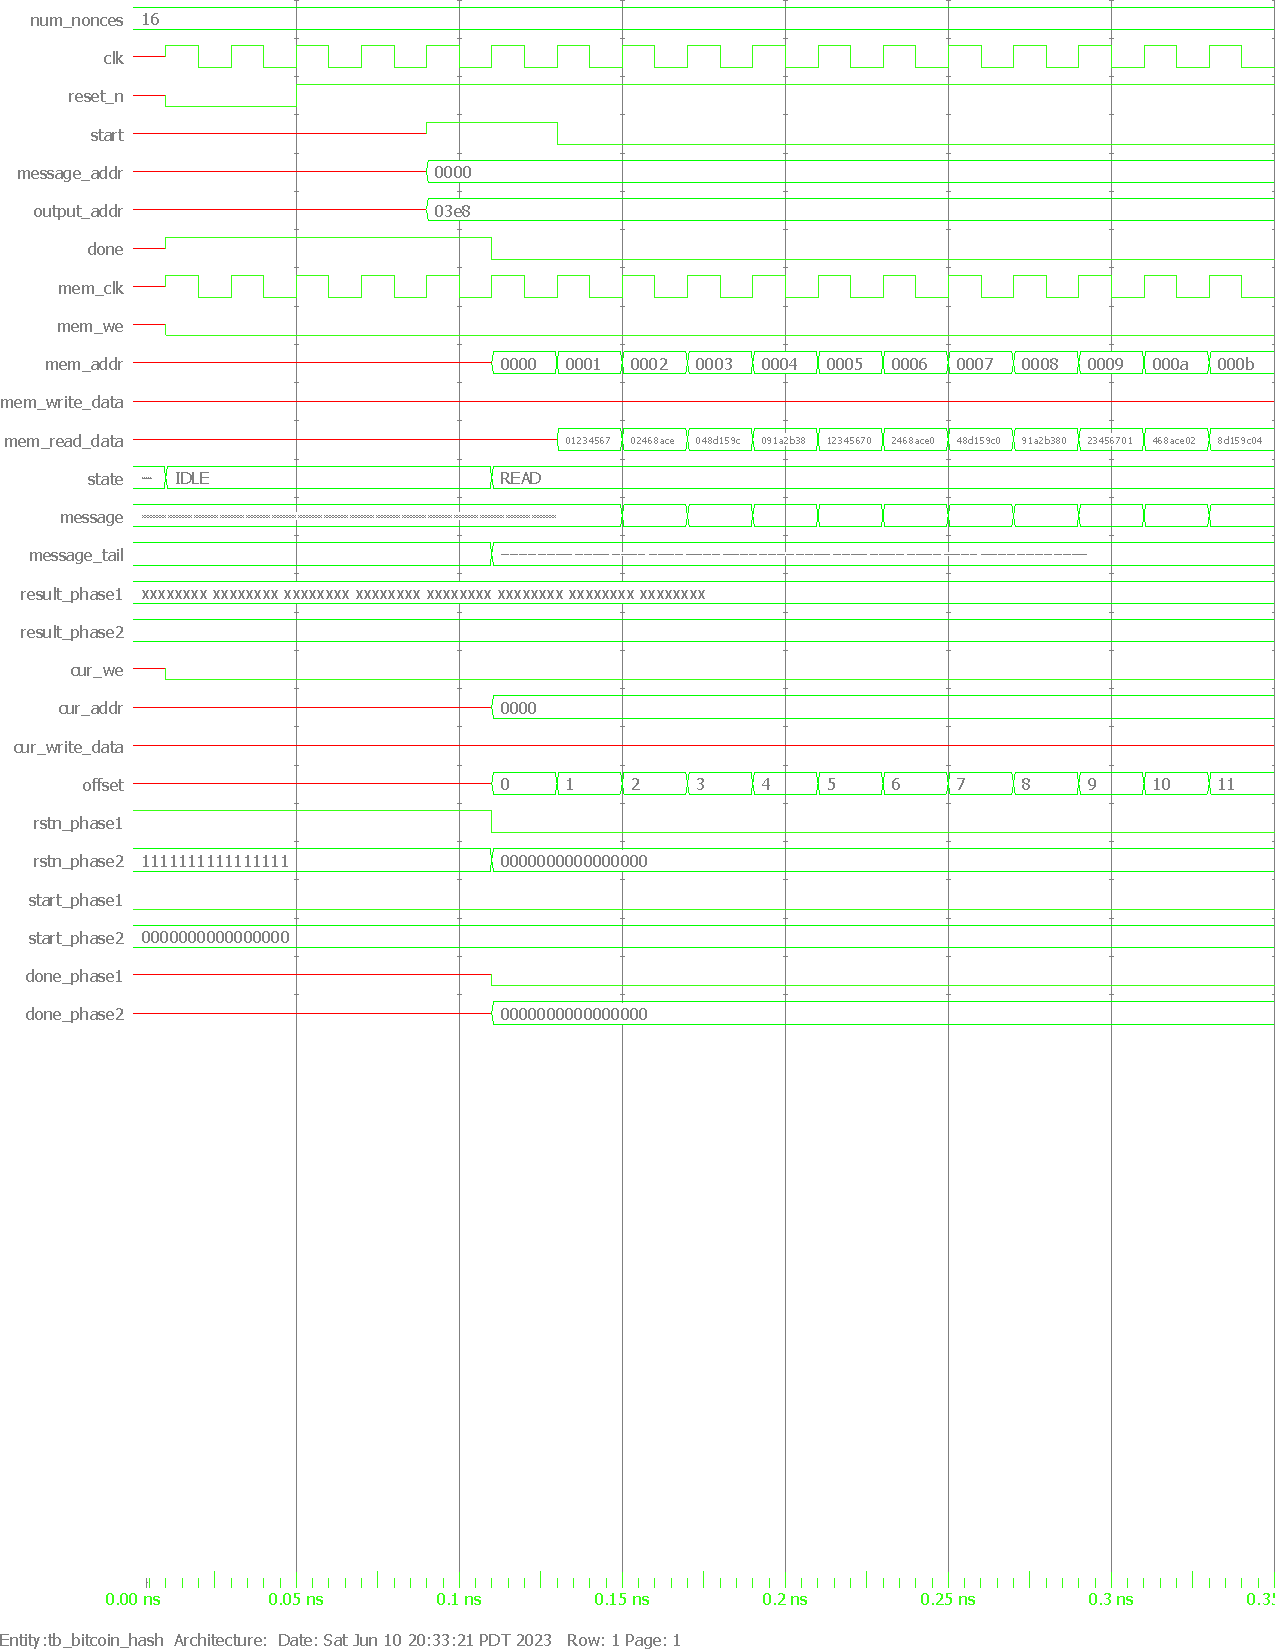
\includepdf[pages=1, pagecommand={\subsection{Bitcoin Hashing} \pagestyle{fancy}}, noautoscale = true,scale=.75]{2wave bit hash.pdf}

\includepdf[pages=2-14, pagecommand={\pagestyle{fancy}}, noautoscale = true,scale=.8]{2wave bit hash.pdf}

\includepdf[pages=15, pagecommand={\label{LastPage} \pagestyle{fancy}}, noautoscale = true,scale=.8]{2wave bit hash.pdf}



\end{document}
